%%%%%%%%%%%%%%%%%%%%%%%%%%%%%%%%%%%%%
%	META DATA						%
%%%%%%%%%%%%%%%%%%%%%%%%%%%%%%%%%%%%%

\documentclass[10pt, fleqn]{scrartcl}
\usepackage[T1]{fontenc}
\usepackage[utf8]{inputenc}
\usepackage{nameref}
\usepackage{comment}
\usepackage{textcomp}
\usepackage[a4paper, width=160mm, top=25mm, bottom=25mm]{geometry}
\usepackage[ngerman]{babel}
\usepackage{graphicx}
\usepackage{tikz, pgfplots}
\usepackage{circuitikz}
\usepackage{acronym}
\usepackage{subcaption}
\usepackage{booktabs}
\usepackage{mathtools}
\usepackage{amsmath}
\usepackage{amssymb}
\usepackage{amsthm}
\usepackage{mhchem}
\usepackage{listings}
\usepackage{subfiles}
\usepackage{blindtext}
\usepackage{csquotes}
\usepackage{verbatim}
\usepackage{siunitx}
\usepackage{url}
\usepackage[nottoc]{tocbibind}
\usepackage{fancyhdr}			
\usepackage{enumerate} 
\usepackage[shortlabels]{enumitem}
\usepackage{color}
\usepackage{hyperref}

%%%	Custom commands	%%%

\usepackage[
    left = \glqq{}, 
    right = \grqq{},
    leftsub = \glq{},
    rightsub = \grq{}
]{dirtytalk}


\newcommand{\columnvector}[1]
	{\begin{pmatrix}#1\end{pmatrix}
}

\DeclarePairedDelimiter\abs{\lvert}{\rvert}%

%%% Colors and code %%%

\definecolor{lightgray}{rgb}{.9,.9,.9}
\definecolor{darkgray}{rgb}{.4,.4,.4}
\definecolor{purple}{rgb}{0.65, 0.12, 0.82}
\lstdefinelanguage{JavaScript}{
  keywords={break, case, catch, continue, debugger, default, delete, do, else, false, finally, for, function, if, in, instanceof, new, null, return, switch, this, throw, true, try, typeof, var, void, while, with},
  morecomment=[l]{//},
  morecomment=[s]{/*}{*/},
  morestring=[b]',
  morestring=[b]",
  ndkeywords={class, export, boolean, throw, implements, import, this},
  keywordstyle=\color{blue}\bfseries,
  ndkeywordstyle=\color{darkgray}\bfseries,
  identifierstyle=\color{black},
  commentstyle=\color{purple}\ttfamily,
  stringstyle=\color{red}\ttfamily,
  sensitive=true
}

\lstset{
   language=JavaScript,
   backgroundcolor=\color{lightgray},
   extendedchars=true,
   basicstyle=\footnotesize\ttfamily,
   showstringspaces=false,
   showspaces=false,
   numbers=left,
   numberstyle=\footnotesize,
   numbersep=9pt,
   tabsize=2,
   breaklines=true,
   showtabs=false,
   captionpos=b
}

%%% Graphics and plots %%%

\graphicspath{{images/}}

%%% Header and footer %%%

\pagestyle{fancy}
\fancyhead[l]{Maximilian Kautzsch}
\fancyhead[c]{Dokumentation des Quiz-Projekts}
\fancyhead[r]{18. April 2024}
\fancyfoot[c]{\thepage}
\renewcommand{\headrulewidth}{0.2pt}
\setlength{\headheight}{15pt}

%%% Title page %%%

\begin{titlepage}
\title{Dokumentation des Projekts \glqq{}Quiz zur Topographie Sachsens\grqq{}}
\date{18. April 2024}
\author{Maximilian Kautzsch
	\\ Geschwister-Scholl-Gymnasium Freiberg 
	\\ Klasse 10/3}	
\end{titlepage}

%%% Bibliography input %%%

\usepackage[
	backend=biber,
	style=alphabetic-verb,
]{biblatex}
\addbibresource{references.bib}

%%%%%%%%%%%%%%%%%%%%%%%%%%%%%%%%%%%%%
%	DOCUMENT						%
%%%%%%%%%%%%%%%%%%%%%%%%%%%%%%%%%%%%%

\begin{document}

\maketitle

%%%%%%%%%%%%%%%%%%%%%%%%%%%%%%%%%%%%%
%	METHODEN						%
%%%%%%%%%%%%%%%%%%%%%%%%%%%%%%%%%%%%%

\section{Dokumentation der verwendeten Methoden}

In dieser JavaScript-Datei wurden insgesamt sechs Funktionen geschrieben. Um einen Überblick zu gewinnen, soll im Nachfolgenden jede Methode kurz beschrieben werden.

\subsection{\texttt{showQuetions(index)}}
Zeigt die Fragen und Optionen basierend auf dem angegebenen Index an.

\subsubsection*{Syntax}
\begin{lstlisting}
	showQuetions(index);
\end{lstlisting}

\subsubsection*{Parameter}
\begin{itemize}
	\item \textit{index}: Index der Frage, die angezeigt werden soll
\end{itemize}

\subsection{\texttt{optionSelected(answer)}}
Verarbeitet die vom Benutzer ausgewählte Option und aktualisiert das Spiel entsprechend. Die im Quiz verwendeten Bilder wurden mit Hilfe einer physischen stummen Karte Sachsens erstellt \cite{diercke:map}.

\subsubsection*{Syntax}
\begin{lstlisting}
	optionSelected(answer);
\end{lstlisting}

\subsubsection*{Parameter}
\begin{itemize}
	\item \textit{answer}: Die vom Benutzer ausgewählte Antwortoption
\end{itemize}

\subsection{\texttt{showResult()}}
Zeigt das Endergebnis des Quiz an, einschließlich der Anzahl der richtigen Antworten.

\subsubsection*{Detaillierte Beschreibung}

Die Funktion \texttt{showResult()} wird aufgerufen, wenn das Quiz beendet ist und zeigt das Endergebnis des Quiz an.
Zuerst werden die verschiedenen HTML-Boxen angepasst, um die Ergebnisbox anzuzeigen und die Quiz-Box auszublenden.
Dann wird überprüft, wie viele Fragen der Benutzer richtig beantwortet hat, und entsprechend wird eine Nachricht generiert und angezeigt.
Je nach Punktzahl wird dem Benutzer entweder gratuliert oder ermutigt, es beim nächsten Mal besser zu machen:
\begin{itemize}
	\item Mehr als 3 richtige Antworten: Es wird eine sehr gute Nachricht angezeigt, was auf eine hervorragende Leistung hinweist.
	\item Score zwischen 1 und 3: Eine gute Nachricht wird angezeigt, was bedeutet, dass die Leistung positiv war, aber noch Raum für Verbesserung besteht.
	\item Score von weniger als 1: Es wird eine eher schlechte Nachricht angezeigt, was darauf hindeutet, dass die Leistung verbessert werden muss.
\end{itemize}

Bei der Ausgabe des Punktestands wird auf die Länge des \texttt{questions[]}-Arrays zugegriffen, um einen Anteil der richtigen Antworten an der Anzahl an Fragen zu bilden.

\subsubsection*{Syntax}
\begin{lstlisting}
	showResult();
\end{lstlisting}

\subsection{\texttt{startTimer(time)}}
Startet den Timer für das Quiz.

\subsubsection*{Syntax}
\begin{lstlisting}
	startTimer(time);
\end{lstlisting}

\subsubsection*{Parameter}
\begin{itemize}
	\item \textit{time}: Die Zeit, die für den Timer festgelegt werden soll
\end{itemize}

\subsection{\texttt{startTimerLine(time)}}
Startet die Timerleiste, um den Fortschritt des Timers visuell darzustellen.

\subsubsection*{Syntax}
\begin{lstlisting}
	startTimerLine(time);
\end{lstlisting}

\subsubsection*{Parameter}
\begin{itemize}
	\item \textit{time}: Der aktuelle Zeitwert für die Timerleiste
\end{itemize}

\subsection{\texttt{queCounter(index)}}
Aktualisiert den Fragenzähler, um die aktuelle Fragenummer anzuzeigen.

\subsubsection*{Syntax}
\begin{lstlisting}
	queCounter(index);
\end{lstlisting}

\subsubsection*{Parameter}
\begin{itemize}
	\item \textit{index}: Die Nummer der aktuellen Frage
\end{itemize}

%%%%%%%%%%%%%%%%%%%%%%%%%%%%%%%%%%%%%
%	LOGIK							%
%%%%%%%%%%%%%%%%%%%%%%%%%%%%%%%%%%%%%

\newpage

\section{Beschreibung der Logik des Programms}

\subsection{Hauptalgorithmus}

In der digitalen Welt, wo Interaktivität und Benutzerfreundlichkeit im Vordergrund stehen, ist die klare Darstellung von Programmabläufen unerlässlich. Ein solches Beispiel ist das Flussdiagramm eines Quiz-Programms, das nicht nur die technische Logik, sondern auch die Benutzererfahrung widerspiegelt. In diesem Text werde ich die Logik dieses Programms anhand des bereitgestellten Flussdiagramms (Abbildung \ref{fig:main-logic}) detailliert erläutern.

Das Programm beginnt mit einem simplen Startpunkt, der als Einladung an den Benutzer dient, sich auf das bevorstehende Quiz einzulassen. Unmittelbar darauf folgt die Anzeige von Informationen, die als eine Art Begrüßungsbildschirm fungieren kann, auf dem die Spielregeln oder interessante Fakten zum Quiz präsentiert werden. Diese Phase ist entscheidend, da sie den ersten Eindruck des Benutzers prägt und das Interesse weckt.

Nach der Informationsanzeige steht der Spieler vor einer Entscheidung: Soll das Quiz gestartet werden? Diese Entscheidung ist interaktiv gestaltet, sodass der Spieler aktiv in den Prozess eingebunden wird. Entscheidet sich der Spieler gegen den Start, wird er erneut zur Informationsanzeige geleitet – ein Kreislauf, der Geduld und Flexibilität seitens des Programms zeigt.

Entscheidet sich der Spieler jedoch für "Ja", beginnt das eigentliche Herzstück des Programms – das Quiz. Eine Frage wird angezeigt, und der Spieler muss innerhalb einer vorgegebenen Zeit eine Antwort auswählen. Diese Phase ist geprägt von Spannung und Schnelligkeit, da der Spieler unter Zeitdruck steht. Läuft die Zeit ab, ohne dass eine Antwort ausgewählt wurde, endet die Frage mit der Anzeige des Resultats. Wurde jedoch eine Antwort ausgewählt, prüft das Programm, ob es sich um die letzte Frage handelt oder ob weitere Fragen folgen.

Ist die aktuelle Frage die letzte, wird das Resultat des gesamten Quiz angezeigt. Sind jedoch weitere Fragen vorhanden, wird die nächste Frage präsentiert. Dieser Zyklus aus Frage und Antwort setzt sich fort, bis alle Fragen beantwortet sind. Das Resultat bietet dem Spieler eine Rückmeldung über seine Leistung und kann als Motivation dienen, sich zu verbessern oder das Gelernte zu festigen.

Nach Abschluss des Quiz steht der Spieler vor einer weiteren Entscheidung: Soll das Quiz wiederholt oder beendet werden? Die Option, das Quiz zu wiederholen, ermöglicht es dem Spieler, aus Fehlern zu lernen und sich zu verbessern. Die Option, das Quiz zu beenden, führt zum Ende des Programms. Dieser letzte Schritt symbolisiert den Abschluss eines Lernzyklus und gibt dem Spieler die Kontrolle über seine Lernerfahrung.

\subsection{Zählen der richtigen Antworten}

Zu Beginn erfolgt die Initialisierungsphase, in der alle notwendigen Variablen und Zustände für das Quiz festgelegt werden. Diese umfasst beispielsweise das Zurücksetzen des Zählers für die richtigen Antworten und das Abrufen der ausgewählten Option des Users sowie der richtigen Antwort aus dem \texttt{questions[]}-Array (Abb. \ref{fig:counting-mechanism}).

Sobald die Initialisierung abgeschlossen ist, stellt das Programm die zentrale Frage: Wurde eine Frage beantwortet? Diese Entscheidungsschleife ist das Herzstück des Programms, da sie bestimmt, wie das Programm auf Benutzereingaben reagiert. Wenn keine Antwort gegeben wurde, kehrt das Programm zur Initialisierungsphase zurück, um auf die nächste Aktion des Benutzers zu warten. Dies gewährleistet, dass das Programm in einem bereiten Zustand bleibt und auf die Interaktion des Benutzers reagieren kann.

Wurde jedoch eine Antwort gegeben, prüft das Programm, ob diese Antwort richtig ist. Diese Überprüfung ist entscheidend, da sie die Genauigkeit des Quiz sicherstellt. Bei einer richtigen Antwort wird der Zähler für die richtigen Ergebnisse erhöht und die Box der korrekten Antwort erhält einen grünen Hintergrund. Dieser Schritt ist ein wesentlicher Bestandteil des Feedback-Mechanismus, der dem Benutzer eine direkte Rückmeldung über seine Leistung gibt \cite{renaud:feedback}.

Ist die Antwort jedoch falsch oder wurde der Zähler bereits erhöht, wird zunächst die richtige Antwort grün markiert und das Programm geht weiter zur nächsten Frage. Dieser Übergang ist nahtlos und stellt sicher, dass das Quiz ohne Unterbrechung fortgesetzt wird. Die Schleife, die von der Überprüfung der Antwort zurück zur zentralen Frage führt, ermöglicht es dem Programm, durch das gesamte Quiz zu navigieren, bis alle Fragen beantwortet wurden.

\subsection{Auswertung der Ergebnisse}

Zunächst startet die Funktion mit einer Initialisierungsphase, in der das System vorbereitet wird, um die Ergebnisse des Benutzers zu empfangen und zu verarbeiten. Diese Phase beinhaltet das Ausblenden der Info-Box und Quiz-Box sowie das Anzeigen der Ergebnis-Box (Abb. \ref{fig:presenting-results}).

Nach der Initialisierung tritt das Programm in die entscheidende Phase der Score-Überprüfung ein. Hier wird der vom Benutzer erzielte Score mit festgelegten Schwellenwerten verglichen, um die Qualität der Leistung zu bestimmen. Abhängig vom Ergebnis dieses Vergleichs wird eine von drei Nachrichten angezeigt: eine gute, eine mittlere oder eine schlechte Nachricht.

Wenn der Score des Benutzers größer als drei ist, zeigt das Programm eine gute Nachricht an. Diese Nachricht könnte eine Gratulation oder eine positive Rückmeldung enthalten, die den Benutzer für seine hervorragende Leistung lobt. Es ist ein Moment der Anerkennung und des Erfolgs, der den Benutzer motivieren soll, weiterhin gute Leistungen zu erbringen.

Liegt der Score zwischen einschließlich zwei und drei, wird eine mittlere Nachricht angezeigt. Diese Nachricht ist wahrscheinlich konstruktiv und ermutigend, weist aber darauf hin, dass noch Raum für Verbesserungen besteht. Sie dient dazu, den Benutzer anzuspornen, sich weiter anzustrengen und seine Fähigkeiten zu verbessern.

Ist der Score jedoch gleich oder kleiner als eins, wird eine schlechte Nachricht präsentiert. Diese Nachricht könnte Hinweise auf Bereiche enthalten, die einer Verbesserung bedürfen, und bietet möglicherweise Ratschläge oder Ressourcen zur Unterstützung des Benutzers bei der Verbesserung seiner Leistung.

Unabhängig von der Art der Nachricht, die angezeigt wird, führen alle Wege zum Ende der Funktion.

%%%%%%%%%%%%%%%%%%%%%%%%%%%%%%%%%%%%%
%	TESTDURCHLAUF					%
%%%%%%%%%%%%%%%%%%%%%%%%%%%%%%%%%%%%%

\newpage

\section{Testdurchlauf}

Testdurchlauf durch:
\noindent\null
\rule{11.5cm}{.4pt} \\

\noindent\hspace*{7cm}
Name, Vorname \\
\vspace{1cm}

\noindent\null
Notiere deine Eindrücke und Feststellungen in maximal drei Stichpunkten:

\begin{itemize}
	\item \noindent\null\rule{14cm}{.4pt} \\
		  \vspace{0.1cm} \\
		  \noindent\null\rule{14cm}{.4pt} \\
	\item \noindent\null\rule{14cm}{.4pt} \\
		  \vspace{0.1cm} \\
		  \noindent\null\rule{14cm}{.4pt} \\
	\item \noindent\null\rule{14cm}{.4pt} \\
		  \vspace{0.1cm} \\
		  \noindent\null\rule{14cm}{.4pt} \\
\end{itemize}

%%%%%%%%%%%%%%%%%%%%%%%%%%%%%%%%%%%%%
%	AUSWERTUNG						%
%%%%%%%%%%%%%%%%%%%%%%%%%%%%%%%%%%%%%

\newpage

\section{Auswertung}

\begin{figure}[h!]
	\centering
	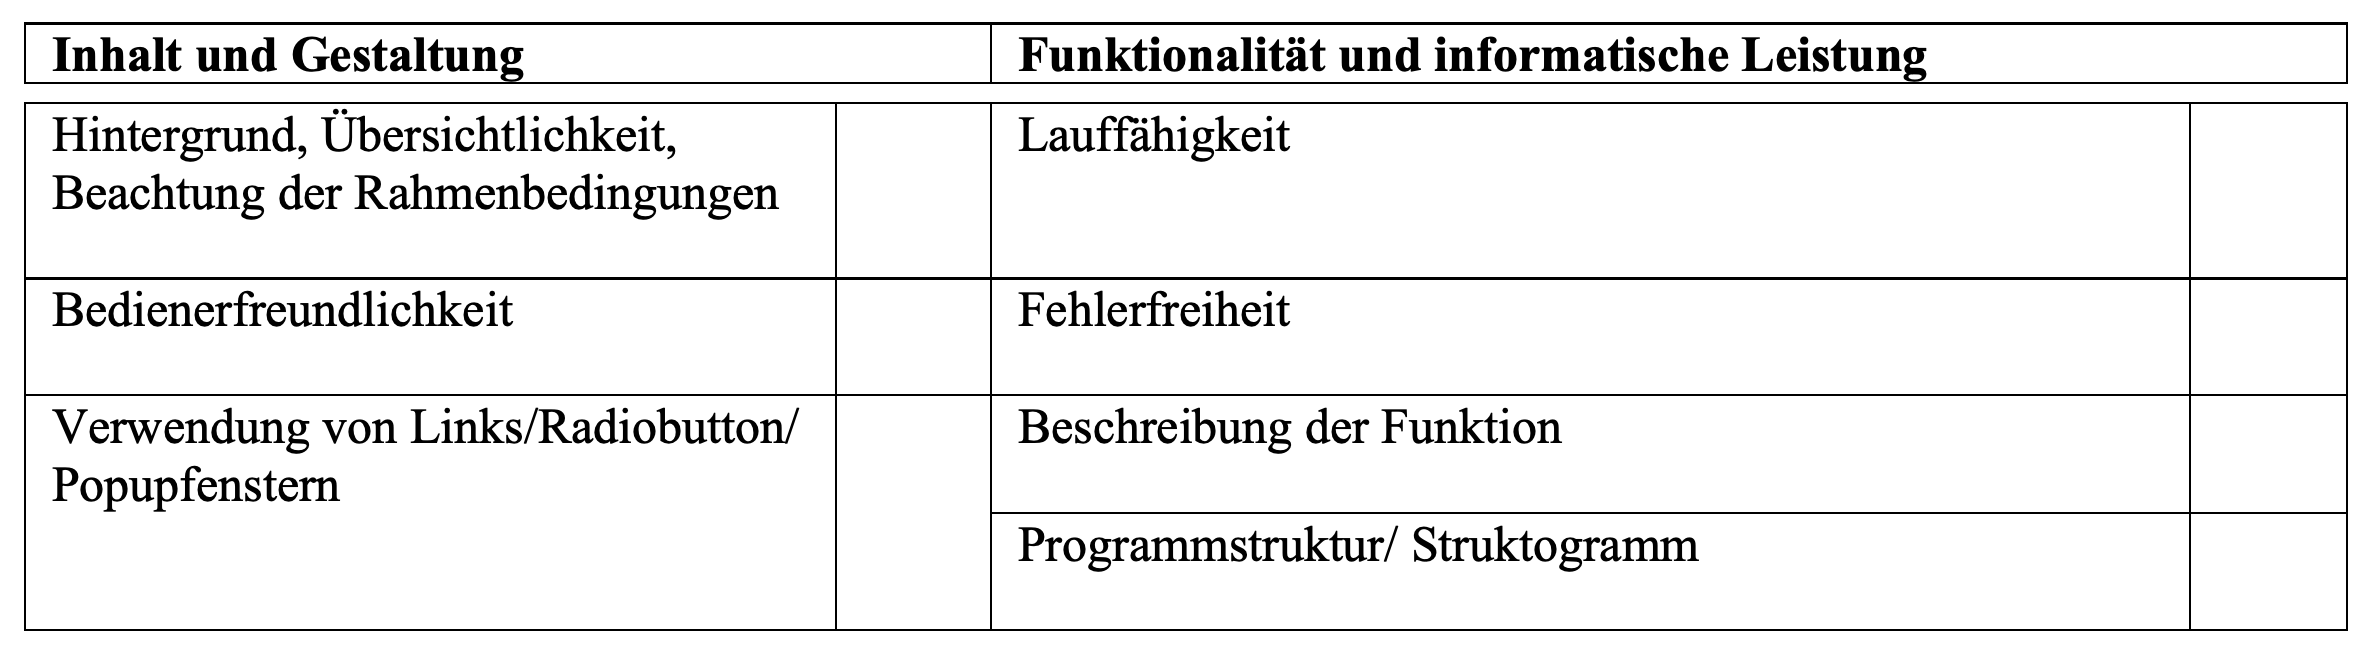
\includegraphics[width=\textwidth]{tables/evaluation.png}
	\label{table:evaluation}
\end{figure}

\noindent
\vspace{1cm} \\
Note:

%%%%%%%%%%%%%%%%%%%%%%%%%%%%%%%%%%%%%
%	LITERATUR						%
%%%%%%%%%%%%%%%%%%%%%%%%%%%%%%%%%%%%%

\newpage

\printbibliography

%%%%%%%%%%%%%%%%%%%%%%%%%%%%%%%%%%%%%
%	APPENDIX						%
%%%%%%%%%%%%%%%%%%%%%%%%%%%%%%%%%%%%%

\newpage

\appendix

\section{Appendix}

\begin{figure}[h!]
	\centering
	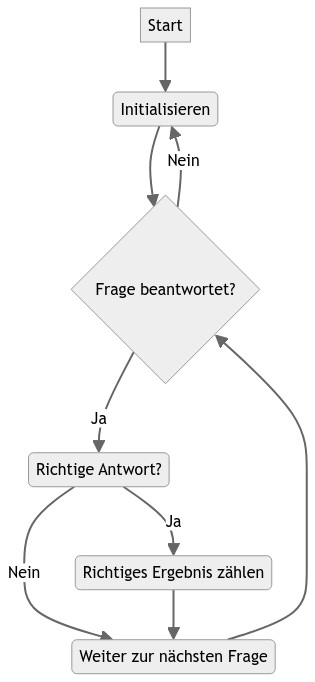
\includegraphics[scale=0.4]{flowcharts/flowchart2.png}
	\caption{Präzisionsmechanismus zur Auswertung von Quizantworten: Ein systematischer Ansatz zur Erfassung und Bewertung der Benutzerleistung im interaktiven Quizkontext.}
	\label{fig:counting-mechanism}
\end{figure}

\begin{figure}[h!]
	\centering
	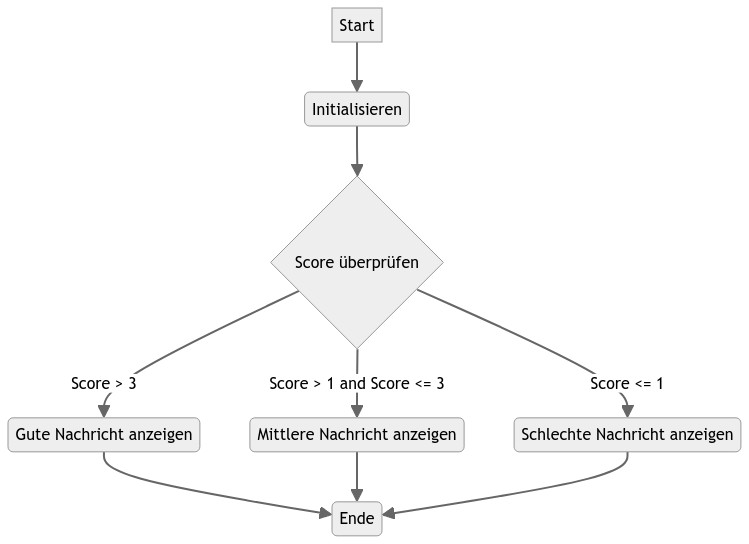
\includegraphics[scale=0.4]{flowcharts/flowchart3.png}
	\caption{Stufenweise Bewertung und differenziertes Feedback: Ein Flussdiagramm, das den Prozess der Leistungsauswertung und die darauf basierende individuelle Rückmeldung im Bildungskontext visualisiert.}
	\label{fig:presenting-results}
\end{figure}

\begin{figure}[h!]
	\centering
	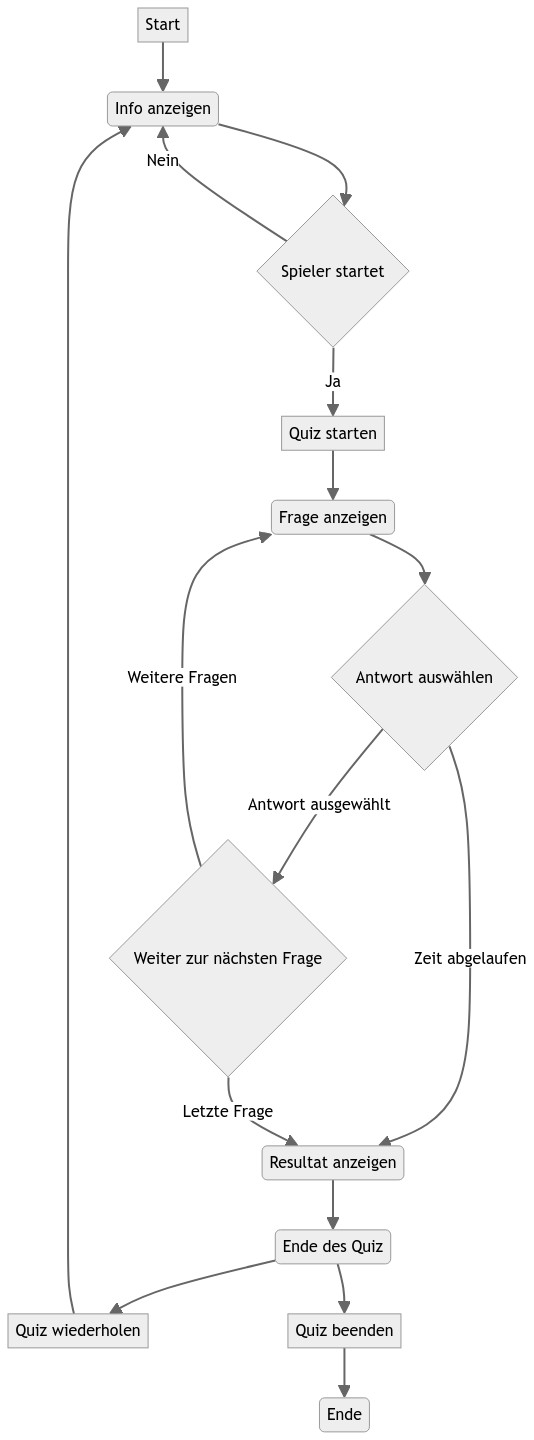
\includegraphics[scale=0.4]{flowcharts/flowchart1.png}
	\caption{Interaktiver Ablauf des Quiz-Programms: Von der Benutzerführung bis zur Ergebnispräsentation – ein Wegweiser durch die digitale Lernerfahrung.}
	\label{fig:main-logic}
\end{figure}

\end{document}